% !TEX TS-program = pdflatex
% !TEX encoding = UTF-8 Unicode
\documentclass[border=0mm]{standalone}
% packages
\usepackage{tikz}
\usetikzlibrary{patterns}
\usepackage{amsmath,amssymb}
\usepackage{bm}
\usepackage{pgfplots}
\pgfplotsset{compat=1.15}
% start document
\begin{document}
% generated by ROOT (CERN)
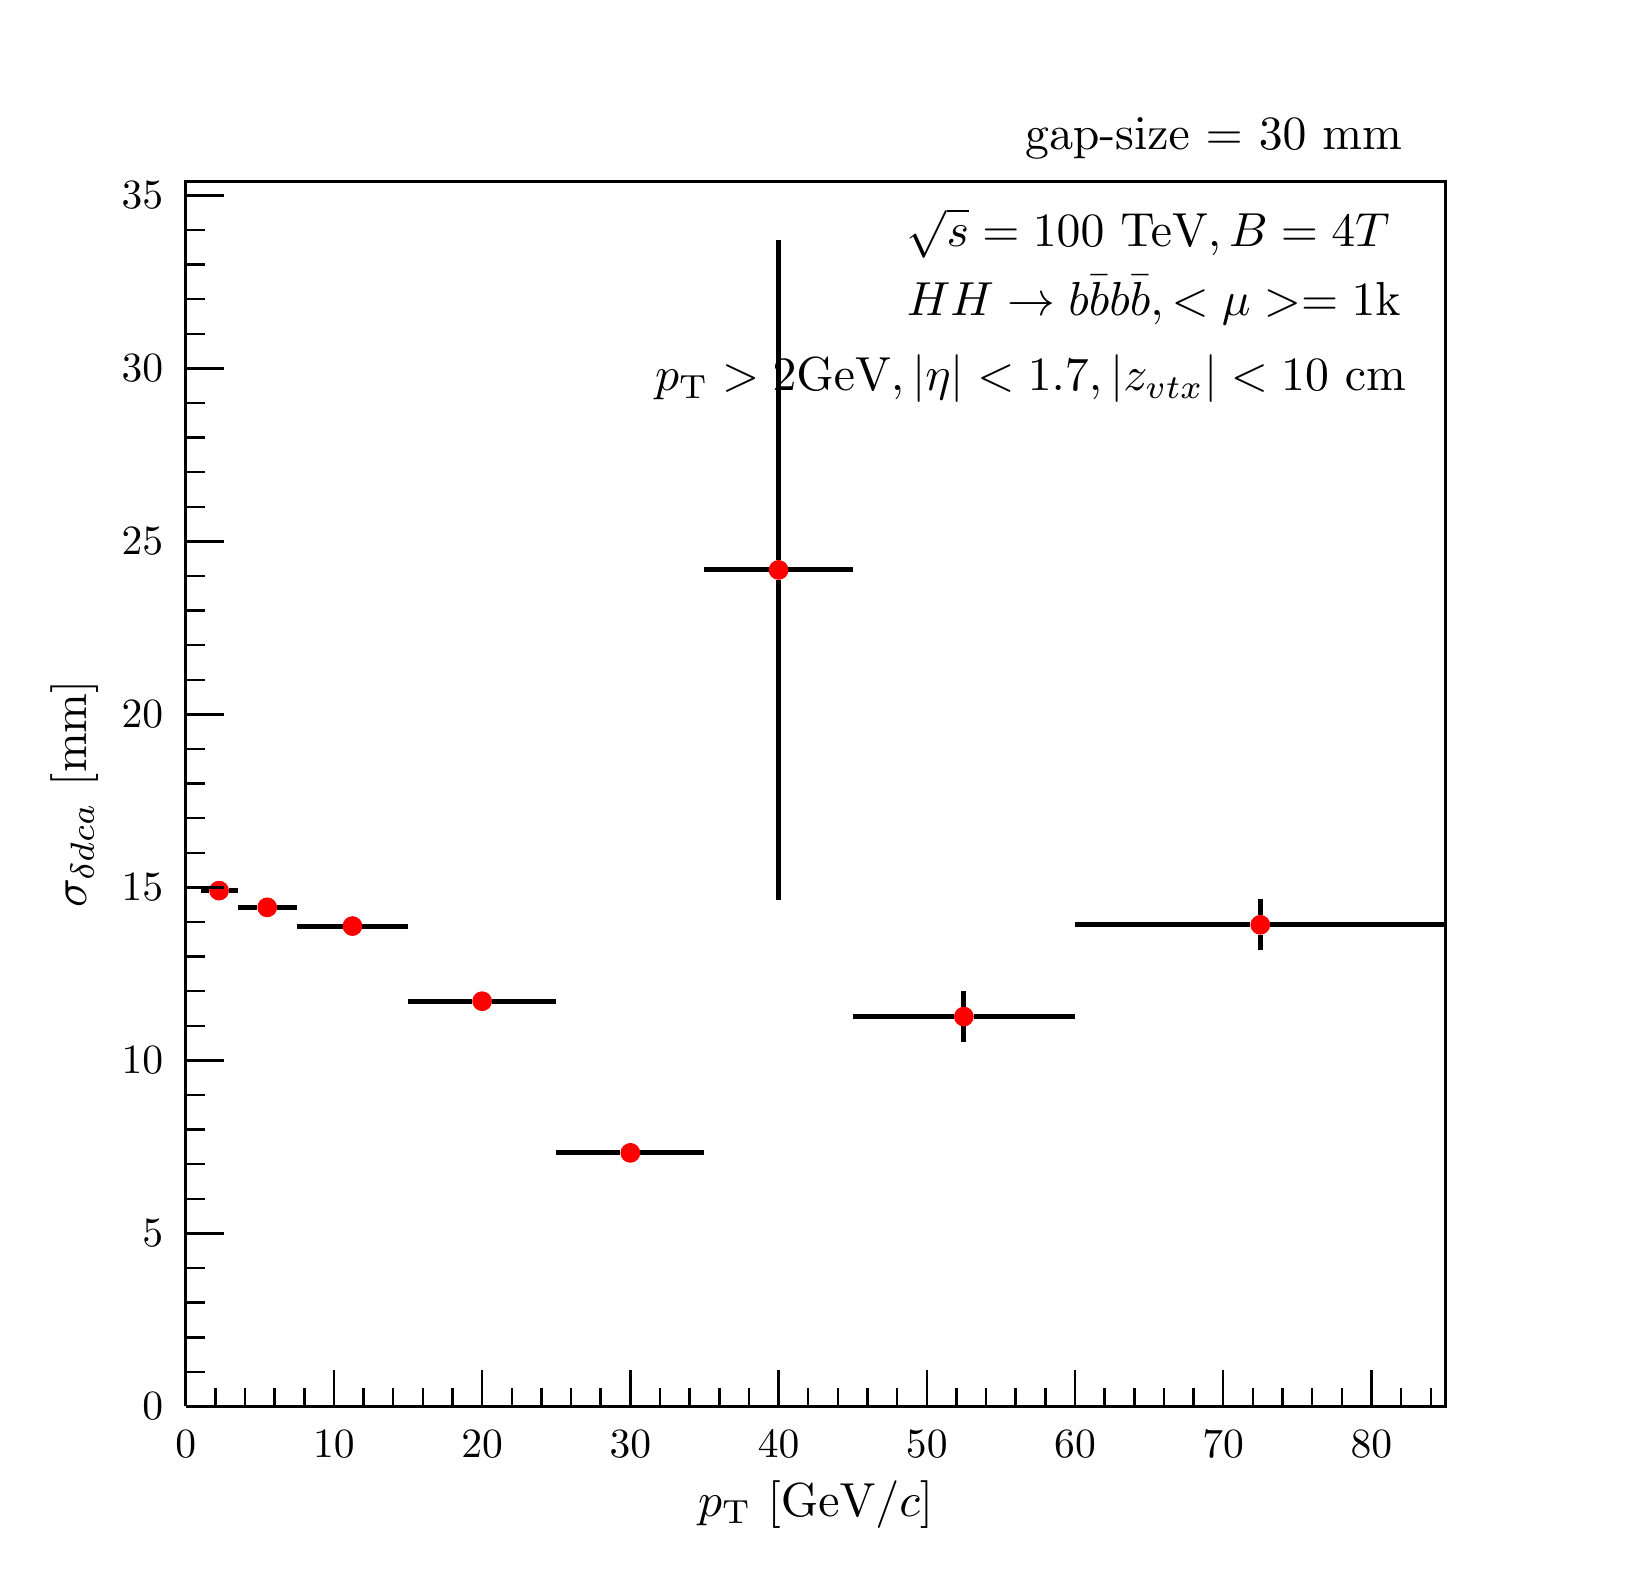
\begin{tikzpicture}
\pgfdeclareplotmark{cross} {
\pgfpathmoveto{\pgfpoint{-0.3\pgfplotmarksize}{\pgfplotmarksize}}
\pgfpathlineto{\pgfpoint{+0.3\pgfplotmarksize}{\pgfplotmarksize}}
\pgfpathlineto{\pgfpoint{+0.3\pgfplotmarksize}{0.3\pgfplotmarksize}}
\pgfpathlineto{\pgfpoint{+1\pgfplotmarksize}{0.3\pgfplotmarksize}}
\pgfpathlineto{\pgfpoint{+1\pgfplotmarksize}{-0.3\pgfplotmarksize}}
\pgfpathlineto{\pgfpoint{+0.3\pgfplotmarksize}{-0.3\pgfplotmarksize}}
\pgfpathlineto{\pgfpoint{+0.3\pgfplotmarksize}{-1.\pgfplotmarksize}}
\pgfpathlineto{\pgfpoint{-0.3\pgfplotmarksize}{-1.\pgfplotmarksize}}
\pgfpathlineto{\pgfpoint{-0.3\pgfplotmarksize}{-0.3\pgfplotmarksize}}
\pgfpathlineto{\pgfpoint{-1.\pgfplotmarksize}{-0.3\pgfplotmarksize}}
\pgfpathlineto{\pgfpoint{-1.\pgfplotmarksize}{0.3\pgfplotmarksize}}
\pgfpathlineto{\pgfpoint{-0.3\pgfplotmarksize}{0.3\pgfplotmarksize}}
\pgfpathclose
\pgfusepathqstroke
}
\pgfdeclareplotmark{cross*} {
\pgfpathmoveto{\pgfpoint{-0.3\pgfplotmarksize}{\pgfplotmarksize}}
\pgfpathlineto{\pgfpoint{+0.3\pgfplotmarksize}{\pgfplotmarksize}}
\pgfpathlineto{\pgfpoint{+0.3\pgfplotmarksize}{0.3\pgfplotmarksize}}
\pgfpathlineto{\pgfpoint{+1\pgfplotmarksize}{0.3\pgfplotmarksize}}
\pgfpathlineto{\pgfpoint{+1\pgfplotmarksize}{-0.3\pgfplotmarksize}}
\pgfpathlineto{\pgfpoint{+0.3\pgfplotmarksize}{-0.3\pgfplotmarksize}}
\pgfpathlineto{\pgfpoint{+0.3\pgfplotmarksize}{-1.\pgfplotmarksize}}
\pgfpathlineto{\pgfpoint{-0.3\pgfplotmarksize}{-1.\pgfplotmarksize}}
\pgfpathlineto{\pgfpoint{-0.3\pgfplotmarksize}{-0.3\pgfplotmarksize}}
\pgfpathlineto{\pgfpoint{-1.\pgfplotmarksize}{-0.3\pgfplotmarksize}}
\pgfpathlineto{\pgfpoint{-1.\pgfplotmarksize}{0.3\pgfplotmarksize}}
\pgfpathlineto{\pgfpoint{-0.3\pgfplotmarksize}{0.3\pgfplotmarksize}}
\pgfpathclose
\pgfusepathqfillstroke
}
\pgfdeclareplotmark{newstar} {
\pgfpathmoveto{\pgfqpoint{0pt}{\pgfplotmarksize}}
\pgfpathlineto{\pgfqpointpolar{44}{0.5\pgfplotmarksize}}
\pgfpathlineto{\pgfqpointpolar{18}{\pgfplotmarksize}}
\pgfpathlineto{\pgfqpointpolar{-20}{0.5\pgfplotmarksize}}
\pgfpathlineto{\pgfqpointpolar{-54}{\pgfplotmarksize}}
\pgfpathlineto{\pgfqpointpolar{-90}{0.5\pgfplotmarksize}}
\pgfpathlineto{\pgfqpointpolar{234}{\pgfplotmarksize}}
\pgfpathlineto{\pgfqpointpolar{198}{0.5\pgfplotmarksize}}
\pgfpathlineto{\pgfqpointpolar{162}{\pgfplotmarksize}}
\pgfpathlineto{\pgfqpointpolar{134}{0.5\pgfplotmarksize}}
\pgfpathclose
\pgfusepathqstroke
}
\pgfdeclareplotmark{newstar*} {
\pgfpathmoveto{\pgfqpoint{0pt}{\pgfplotmarksize}}
\pgfpathlineto{\pgfqpointpolar{44}{0.5\pgfplotmarksize}}
\pgfpathlineto{\pgfqpointpolar{18}{\pgfplotmarksize}}
\pgfpathlineto{\pgfqpointpolar{-20}{0.5\pgfplotmarksize}}
\pgfpathlineto{\pgfqpointpolar{-54}{\pgfplotmarksize}}
\pgfpathlineto{\pgfqpointpolar{-90}{0.5\pgfplotmarksize}}
\pgfpathlineto{\pgfqpointpolar{234}{\pgfplotmarksize}}
\pgfpathlineto{\pgfqpointpolar{198}{0.5\pgfplotmarksize}}
\pgfpathlineto{\pgfqpointpolar{162}{\pgfplotmarksize}}
\pgfpathlineto{\pgfqpointpolar{134}{0.5\pgfplotmarksize}}
\pgfpathclose
\pgfusepathqfillstroke
}
\definecolor{c}{rgb}{1,1,1};
\draw [color=c, fill=c] (0,0) rectangle (20,19.4486);
\draw [color=c, fill=c] (2,1.94486) rectangle (18,17.5038);
\definecolor{c}{rgb}{0,0,0};
\draw [c,line width=0.9] (2,1.94486) -- (2,17.5038) -- (18,17.5038) -- (18,1.94486) -- (2,1.94486);
\draw [c,line width=1.8] (2.18824,8.49615) -- (2.29822,8.49615);
\draw [c,line width=1.8] (2.54884,8.49615) -- (2.65882,8.49615);
\definecolor{c}{rgb}{1,0,0};
\foreach \P in {(2.42353,8.49615)}{\draw[mark options={color=c,fill=c},mark size=3.363363pt,mark=*] plot coordinates {\P};}
\definecolor{c}{rgb}{0,0,0};
\draw [c,line width=1.8] (2.65882,8.28357) -- (2.90998,8.28357);
\draw [c,line width=1.8] (3.16061,8.28357) -- (3.41176,8.28357);
\definecolor{c}{rgb}{1,0,0};
\foreach \P in {(3.03529,8.28357)}{\draw[mark options={color=c,fill=c},mark size=3.363363pt,mark=*] plot coordinates {\P};}
\definecolor{c}{rgb}{0,0,0};
\draw [c,line width=1.8] (3.41176,8.04574) -- (3.99233,8.04574);
\draw [c,line width=1.8] (4.24296,8.04574) -- (4.82353,8.04574);
\definecolor{c}{rgb}{1,0,0};
\foreach \P in {(4.11765,8.04574)}{\draw[mark options={color=c,fill=c},mark size=3.363363pt,mark=*] plot coordinates {\P};}
\definecolor{c}{rgb}{0,0,0};
\draw [c,line width=1.8] (4.82353,7.09164) -- (5.63939,7.09164);
\draw [c,line width=1.8] (5.89002,7.09164) -- (6.70588,7.09164);
\definecolor{c}{rgb}{1,0,0};
\foreach \P in {(5.76471,7.09164)}{\draw[mark options={color=c,fill=c},mark size=3.363363pt,mark=*] plot coordinates {\P};}
\definecolor{c}{rgb}{0,0,0};
\draw [c,line width=1.8] (6.70588,5.16561) -- (7.52175,5.16561);
\draw [c,line width=1.8] (7.77237,5.16561) -- (8.58823,5.16561);
\definecolor{c}{rgb}{1,0,0};
\foreach \P in {(7.64706,5.16561)}{\draw[mark options={color=c,fill=c},mark size=3.363363pt,mark=*] plot coordinates {\P};}
\definecolor{c}{rgb}{0,0,0};
\draw [c,line width=1.8] (9.52941,8.37503) -- (9.52941,12.4436);
\draw [c,line width=1.8] (9.52941,12.6943) -- (9.52941,16.7629);
\draw [c,line width=1.8] (8.58823,12.5689) -- (9.4041,12.5689);
\draw [c,line width=1.8] (9.65473,12.5689) -- (10.4706,12.5689);
\definecolor{c}{rgb}{1,0,0};
\foreach \P in {(9.52941,12.5689)}{\draw[mark options={color=c,fill=c},mark size=3.363363pt,mark=*] plot coordinates {\P};}
\definecolor{c}{rgb}{0,0,0};
\draw [c,line width=1.8] (11.8824,6.57091) -- (11.8824,6.77092);
\draw [c,line width=1.8] (11.8824,7.02155) -- (11.8824,7.22156);
\draw [c,line width=1.8] (10.4706,6.89623) -- (11.757,6.89623);
\draw [c,line width=1.8] (12.0077,6.89623) -- (13.2941,6.89623);
\definecolor{c}{rgb}{1,0,0};
\foreach \P in {(11.8824,6.89623)}{\draw[mark options={color=c,fill=c},mark size=3.363363pt,mark=*] plot coordinates {\P};}
\definecolor{c}{rgb}{0,0,0};
\draw [c,line width=1.8] (15.6471,7.73853) -- (15.6471,7.93661);
\draw [c,line width=1.8] (15.6471,8.18723) -- (15.6471,8.38531);
\draw [c,line width=1.8] (13.2941,8.06192) -- (15.5217,8.06192);
\draw [c,line width=1.8] (15.7724,8.06192) -- (18,8.06192);
\definecolor{c}{rgb}{1,0,0};
\foreach \P in {(15.6471,8.06192)}{\draw[mark options={color=c,fill=c},mark size=3.363363pt,mark=*] plot coordinates {\P};}
\definecolor{c}{rgb}{0,0,0};
\draw [c,line width=0.9] (2,1.94486) -- (18,1.94486);
\draw [c,line width=0.9] (2,2.41163) -- (2,1.94486);
\draw [c,line width=0.9] (2.37647,2.17825) -- (2.37647,1.94486);
\draw [c,line width=0.9] (2.75294,2.17825) -- (2.75294,1.94486);
\draw [c,line width=0.9] (3.12941,2.17825) -- (3.12941,1.94486);
\draw [c,line width=0.9] (3.50588,2.17825) -- (3.50588,1.94486);
\draw [c,line width=0.9] (3.88235,2.41163) -- (3.88235,1.94486);
\draw [c,line width=0.9] (4.25882,2.17825) -- (4.25882,1.94486);
\draw [c,line width=0.9] (4.63529,2.17825) -- (4.63529,1.94486);
\draw [c,line width=0.9] (5.01177,2.17825) -- (5.01177,1.94486);
\draw [c,line width=0.9] (5.38824,2.17825) -- (5.38824,1.94486);
\draw [c,line width=0.9] (5.76471,2.41163) -- (5.76471,1.94486);
\draw [c,line width=0.9] (6.14118,2.17825) -- (6.14118,1.94486);
\draw [c,line width=0.9] (6.51765,2.17825) -- (6.51765,1.94486);
\draw [c,line width=0.9] (6.89412,2.17825) -- (6.89412,1.94486);
\draw [c,line width=0.9] (7.27059,2.17825) -- (7.27059,1.94486);
\draw [c,line width=0.9] (7.64706,2.41163) -- (7.64706,1.94486);
\draw [c,line width=0.9] (8.02353,2.17825) -- (8.02353,1.94486);
\draw [c,line width=0.9] (8.4,2.17825) -- (8.4,1.94486);
\draw [c,line width=0.9] (8.77647,2.17825) -- (8.77647,1.94486);
\draw [c,line width=0.9] (9.15294,2.17825) -- (9.15294,1.94486);
\draw [c,line width=0.9] (9.52941,2.41163) -- (9.52941,1.94486);
\draw [c,line width=0.9] (9.90588,2.17825) -- (9.90588,1.94486);
\draw [c,line width=0.9] (10.2824,2.17825) -- (10.2824,1.94486);
\draw [c,line width=0.9] (10.6588,2.17825) -- (10.6588,1.94486);
\draw [c,line width=0.9] (11.0353,2.17825) -- (11.0353,1.94486);
\draw [c,line width=0.9] (11.4118,2.41163) -- (11.4118,1.94486);
\draw [c,line width=0.9] (11.7882,2.17825) -- (11.7882,1.94486);
\draw [c,line width=0.9] (12.1647,2.17825) -- (12.1647,1.94486);
\draw [c,line width=0.9] (12.5412,2.17825) -- (12.5412,1.94486);
\draw [c,line width=0.9] (12.9176,2.17825) -- (12.9176,1.94486);
\draw [c,line width=0.9] (13.2941,2.41163) -- (13.2941,1.94486);
\draw [c,line width=0.9] (13.6706,2.17825) -- (13.6706,1.94486);
\draw [c,line width=0.9] (14.0471,2.17825) -- (14.0471,1.94486);
\draw [c,line width=0.9] (14.4235,2.17825) -- (14.4235,1.94486);
\draw [c,line width=0.9] (14.8,2.17825) -- (14.8,1.94486);
\draw [c,line width=0.9] (15.1765,2.41163) -- (15.1765,1.94486);
\draw [c,line width=0.9] (15.5529,2.17825) -- (15.5529,1.94486);
\draw [c,line width=0.9] (15.9294,2.17825) -- (15.9294,1.94486);
\draw [c,line width=0.9] (16.3059,2.17825) -- (16.3059,1.94486);
\draw [c,line width=0.9] (16.6824,2.17825) -- (16.6824,1.94486);
\draw [c,line width=0.9] (17.0588,2.41163) -- (17.0588,1.94486);
\draw [c,line width=0.9] (17.0588,2.41163) -- (17.0588,1.94486);
\draw [c,line width=0.9] (17.4353,2.17825) -- (17.4353,1.94486);
\draw [c,line width=0.9] (17.8118,2.17825) -- (17.8118,1.94486);
\draw [anchor=base] (2,1.30306) node[scale=1.50291, color=c, rotate=0]{0};
\draw [anchor=base] (3.88235,1.30306) node[scale=1.50291, color=c, rotate=0]{10};
\draw [anchor=base] (5.76471,1.30306) node[scale=1.50291, color=c, rotate=0]{20};
\draw [anchor=base] (7.64706,1.30306) node[scale=1.50291, color=c, rotate=0]{30};
\draw [anchor=base] (9.52941,1.30306) node[scale=1.50291, color=c, rotate=0]{40};
\draw [anchor=base] (11.4118,1.30306) node[scale=1.50291, color=c, rotate=0]{50};
\draw [anchor=base] (13.2941,1.30306) node[scale=1.50291, color=c, rotate=0]{60};
\draw [anchor=base] (15.1765,1.30306) node[scale=1.50291, color=c, rotate=0]{70};
\draw [anchor=base] (17.0588,1.30306) node[scale=1.50291, color=c, rotate=0]{80};
\draw (10,0.700151) node[scale=1.72557, color=c, rotate=0]{$p_{\text{T}} ~[\text{GeV}/c]$};
\draw [c,line width=0.9] (2,1.94486) -- (2,17.5038);
\draw [c,line width=0.9] (2.48,1.94486) -- (2,1.94486);
\draw [c,line width=0.9] (2.24,2.38431) -- (2,2.38431);
\draw [c,line width=0.9] (2.24,2.82376) -- (2,2.82376);
\draw [c,line width=0.9] (2.24,3.26322) -- (2,3.26322);
\draw [c,line width=0.9] (2.24,3.70267) -- (2,3.70267);
\draw [c,line width=0.9] (2.48,4.14212) -- (2,4.14212);
\draw [c,line width=0.9] (2.24,4.58157) -- (2,4.58157);
\draw [c,line width=0.9] (2.24,5.02102) -- (2,5.02102);
\draw [c,line width=0.9] (2.24,5.46047) -- (2,5.46047);
\draw [c,line width=0.9] (2.24,5.89992) -- (2,5.89992);
\draw [c,line width=0.9] (2.48,6.33937) -- (2,6.33937);
\draw [c,line width=0.9] (2.24,6.77882) -- (2,6.77882);
\draw [c,line width=0.9] (2.24,7.21828) -- (2,7.21828);
\draw [c,line width=0.9] (2.24,7.65773) -- (2,7.65773);
\draw [c,line width=0.9] (2.24,8.09718) -- (2,8.09718);
\draw [c,line width=0.9] (2.48,8.53663) -- (2,8.53663);
\draw [c,line width=0.9] (2.24,8.97608) -- (2,8.97608);
\draw [c,line width=0.9] (2.24,9.41553) -- (2,9.41553);
\draw [c,line width=0.9] (2.24,9.85498) -- (2,9.85498);
\draw [c,line width=0.9] (2.24,10.2944) -- (2,10.2944);
\draw [c,line width=0.9] (2.48,10.7339) -- (2,10.7339);
\draw [c,line width=0.9] (2.24,11.1733) -- (2,11.1733);
\draw [c,line width=0.9] (2.24,11.6128) -- (2,11.6128);
\draw [c,line width=0.9] (2.24,12.0522) -- (2,12.0522);
\draw [c,line width=0.9] (2.24,12.4917) -- (2,12.4917);
\draw [c,line width=0.9] (2.48,12.9311) -- (2,12.9311);
\draw [c,line width=0.9] (2.24,13.3706) -- (2,13.3706);
\draw [c,line width=0.9] (2.24,13.81) -- (2,13.81);
\draw [c,line width=0.9] (2.24,14.2495) -- (2,14.2495);
\draw [c,line width=0.9] (2.24,14.6889) -- (2,14.6889);
\draw [c,line width=0.9] (2.48,15.1284) -- (2,15.1284);
\draw [c,line width=0.9] (2.24,15.5678) -- (2,15.5678);
\draw [c,line width=0.9] (2.24,16.0073) -- (2,16.0073);
\draw [c,line width=0.9] (2.24,16.4467) -- (2,16.4467);
\draw [c,line width=0.9] (2.24,16.8862) -- (2,16.8862);
\draw [c,line width=0.9] (2.48,17.3256) -- (2,17.3256);
\draw [c,line width=0.9] (2.48,17.3256) -- (2,17.3256);
\draw [anchor= east] (1.9,1.94486) node[scale=1.50291, color=c, rotate=0]{0};
\draw [anchor= east] (1.9,4.14212) node[scale=1.50291, color=c, rotate=0]{5};
\draw [anchor= east] (1.9,6.33937) node[scale=1.50291, color=c, rotate=0]{10};
\draw [anchor= east] (1.9,8.53663) node[scale=1.50291, color=c, rotate=0]{15};
\draw [anchor= east] (1.9,10.7339) node[scale=1.50291, color=c, rotate=0]{20};
\draw [anchor= east] (1.9,12.9311) node[scale=1.50291, color=c, rotate=0]{25};
\draw [anchor= east] (1.9,15.1284) node[scale=1.50291, color=c, rotate=0]{30};
\draw [anchor= east] (1.9,17.3256) node[scale=1.50291, color=c, rotate=0]{35};
\draw (0.592,9.72431) node[scale=1.72557, color=c, rotate=90]{$\sigma_{\delta dca} ~[\text{mm}]$};
\draw [anchor=base west] (10.945,16.6748) node[scale=1.72557, color=c, rotate=0]{$\sqrt{s} = 100 ~\text{TeV}, B = 4T$};
\draw [anchor=base west] (10.945,15.7996) node[scale=1.72557, color=c, rotate=0]{$HH \rightarrow b\bar{b}b\bar{b}, <\mu> = \text{1k}$};
\draw [anchor=base east] (17.7105,14.8432) node[scale=1.72557, color=c, rotate=0]{$p_{\text{T}} > 2\text{GeV}, |\eta| < 1.7, |z_{vtx}| < 10\text{~cm}$};
\draw [anchor=base west] (12.445,17.9122) node[scale=1.72557, color=c, rotate=0]{gap-size = 30 mm};
\draw [anchor=base west] (12.445,17.5232) node[scale=1.72557, color=c, rotate=0]{ };
\end{tikzpicture}
% end document
\end{document}
